% DO NOT COMPILE THIS FILE DIRECTLY!
% This is included by the other .tex files.

\begin{frame}[t,plain]
\titlepage
\end{frame}

\begin{frame}
    \frametitle{Content of the presentation}
    \begin{itemize}
        \item What problems are we trying to tackle
        \item MISP Workflows overview
        \item Design of the system \& how it can be extended
    \end{itemize}
\end{frame}

\begin{frame}
    \frametitle{What problems are we trying to tackle}
    \begin{itemize}
        \item Initial idea came from GeekWeek7.5\footnote{\href{https://cyber.gc.ca/en/events/geekweek-75}{Workshop organized by the Canadian Cyber Center}}
        \begin{center}
            
\includegraphics[width=0.3\linewidth]{pictures/geekweek75.jpg}
        \end{center}
        \item Needs:
        \begin{itemize}
            \item Interacting with MISP's behavior
            \item Hooking specific action via callbacks
        \end{itemize}
        \item Use-cases:
        \begin{itemize}
            \item Prevent publication of events not meeting some criterias
            \item Prevent querying thrid-party service (e.g. virustotal) for sensitive information
            \item Send a notification in chat room when new events get published
            \item And much much more..
        \end{itemize}
    \end{itemize}
\end{frame}

\begin{frame}
    \frametitle{Simplistic overview of a Workflow in action}
    \begin{enumerate}
        \item An \textbf{action} is performed in MISP
        \item If there is an \textbf{enabled} Workflow for that \textbf{action}
        \item MISP runs the Workflow
        \item If all went fine, MISP \textbf{continue} to perform the action
        \begin{itemize}
            \item The operation can potentially be cancelled by \texttt{blocking} modules
        \end{itemize}
    \end{enumerate}
\end{frame}

\begin{frame}
    \frametitle{Terminology}
    \begin{enumerate}
        \item \textbf{workflow}: Sequence of actions to be executed
        \item \textbf{execution path}: A path composed of nodes to be executed sequentially
        \item \textbf{trigger}: Starting point of a workflow. Triggers are called when specific actions happen in MISP
        \begin{itemize}
            \item A trigger can only have one workflow and vice-versa
        \end{itemize}
    \end{enumerate}
    \begin{center}
        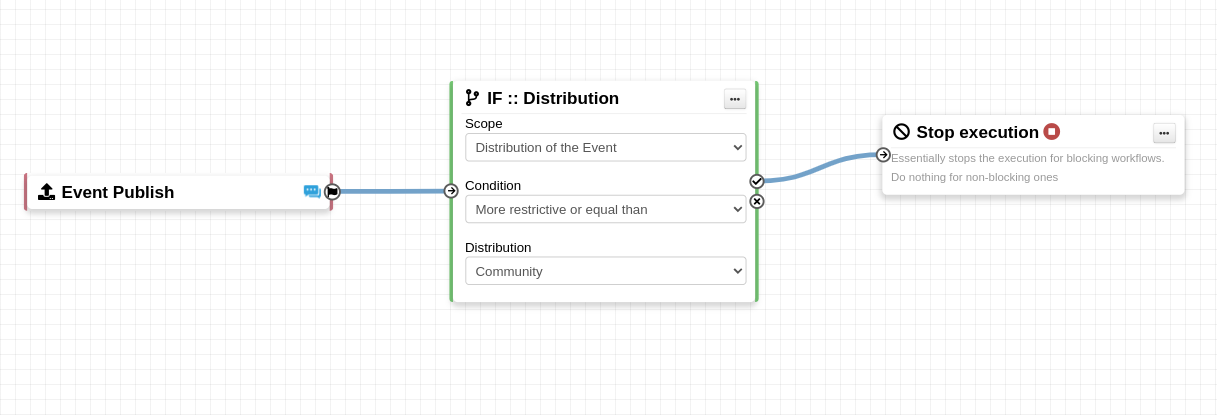
\includegraphics[width=1.0\linewidth]{pictures/simple-workflow.png}
    \end{center}
\end{frame}

\begin{frame}
    \frametitle{Workflow execution process}
    Typical execution process:
    \begin{enumerate}
        \item An action happen in MISP
        \item The workflow associated to the trigger is run
        \item Execution result:
        \begin{itemize}
            \item \texttt{\color{green!50!black}success}: Proceed with the operation
            \item \texttt{\color{red}failure} | \texttt{\color{blue}blocked}: Cancel the operation
        \end{itemize}
    \end{enumerate}
    \vspace{0.5em}
    Example for Event publish:
    \begin{enumerate}
        \item An Event is about to be published
        \item MISP executes the workflow listening to the \texttt{event-publish} trigger
        \begin{itemize}
            \item {\bf\color{green!50!black}success}: Proceed the publishing action
            \item {\bf\color{red}failure} | \texttt{\color{blue}blocked}: Stop publishing and log the reason
        \end{itemize}
    \end{enumerate}
\end{frame}

\begin{frame}
    \frametitle{Blocking and non-blocking Workflows}
    Currently 2 types of workflows:
    \vspace{0.5em}
    \begin{itemize}
        \item {\bf Blocking}: Completion of the initial action can be prevented
        \begin{itemize}
            \item If a \textbf{blocking module} blocks the action
            \item If a \textbf{blocking module} raises an exception
        \end{itemize}
        \vspace{0.5em}
        \item {\bf Non-blocking}: Workflow execution outcome has no impact
        \begin{itemize}
            \item \textbf{Blocking modules} become \textbf{non-blocking}
            \item Execution proceed unless on exception
        \end{itemize}
    \end{itemize}
\end{frame}

\begin{frame}
    \frametitle{Execution context}
    \begin{itemize}
        \item Workflows can be triggered by \textbf{any users}
        \item Workflows can be triggered by operations done via the \textbf{UI or the API}
        \item However, the user for which the workflow executes has the \texttt{site-admin} role and is from the \texttt{MISP.host\_org\_id}
        \item This is to make sure, all data are processed regardless of ownership and access (no ACL)
    \end{itemize}
\end{frame}

\begin{frame}
    \frametitle{Types of Workflow modules}
    \begin{center}
        
\includegraphics[width=0.5\linewidth]{pictures/module-type.png}
    \end{center}
    2 types of action modules
    \begin{itemize}
        \item \textbf{logic}: Allow to redirect the execution flow.
        \begin{itemize}
            \item IF condition, fork the blocking execution into a non-blocking one, ...
        \end{itemize}
        \item \textbf{action}: Allow to perform additional actions, prevent execution or modify data
        \begin{itemize}
            \item Webhook, block the execution, perform enrichments, ...
        \end{itemize}
    \end{itemize}
\end{frame}

\begin{frame}
    \frametitle{Workflow modules}
    3 sources of action modules
    \begin{itemize}
        \item \texttt{\scriptsize app/Model/WorkflowModules/action/[module\_name].php}
        \begin{itemize}
            \item Built-in \textbf{default} modules in the application
            \item Written in PHP
            \item Can use MISP's built-in functionalities (restsearch, enrichment, push to zmq, ...)
            \item Fast and easier to interact with for those having internal knowledge of MISP
        \end{itemize}
        \item \texttt{\scriptsize app/Lib/WorkflowModules/action/[module\_name].php}
        \begin{itemize}
            \item \textbf{Custom} modules written by users
        \end{itemize}
        \item \texttt{From the misp-module service} 
        \begin{itemize}
            \item \textbf{Default} and \textbf{custom} modules
            \item Written in Python
            \item Can use any python libraries
            \item New \texttt{misp-module} module type: \texttt{action}
        \end{itemize}
    \end{itemize}
    \begin{center}
        $\rightarrow$ Both the PHP and Python systems are \textbf{plug-and-play}
    \end{center}
\end{frame}

\begin{frame}
    \frametitle{Getting started with workflows (1)}
    Review MISP settings:
    \begin{enumerate}
        \item Make sure \texttt{MISP.background\_jobs} is turned on
        \item Turn on setting \texttt{Plugin.Workflow\_enable}
        \item Make sure workers are up-and-running and healthy
    \end{enumerate}
    \begin{center}
        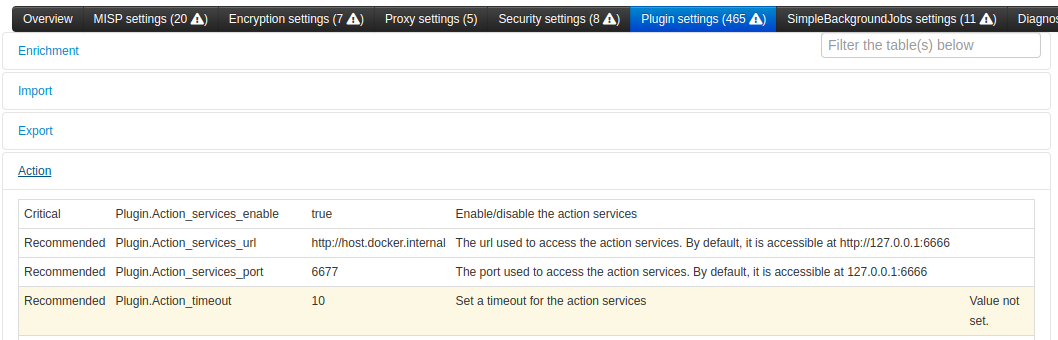
\includegraphics[width=0.75\linewidth]{pictures/settings-1.png}
        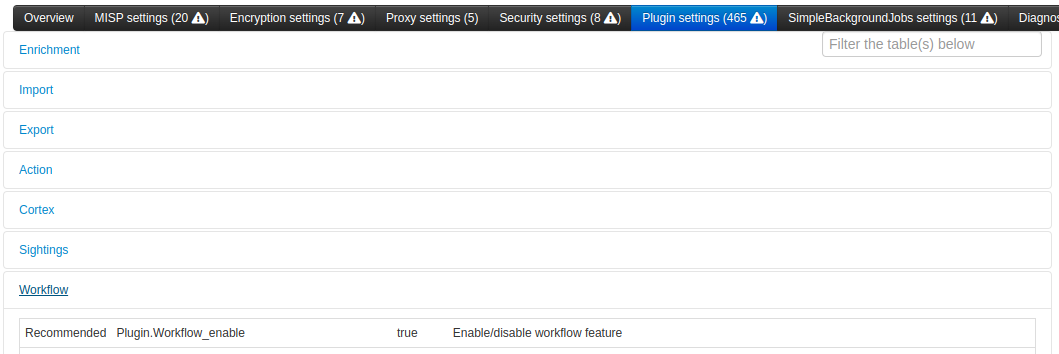
\includegraphics[width=0.75\linewidth]{pictures/settings-2.png}
    \end{center}
\end{frame}

\begin{frame}
    \frametitle{Getting started with workflows (2)}
    If you wish to use action modules from \texttt{misp-module}:
    \begin{itemize}
        \item Make sure you update your \texttt{misp-module} application to the latest version
        \item Make sure your have the new \texttt{action\_mod} module type in \url{misp-modules/misp\_modules/modules}
        \item Restart your \texttt{misp-module} application
    \end{itemize}
\end{frame}

\begin{frame}
    \frametitle{Getting started with workflows (3)}
    \begin{enumerate}
        \item Go to the trigger list: \texttt{Administration > Workflows}
        \begin{itemize}
            \item \url{/workflows/triggers}
        \end{itemize}
        \item Turn a trigger on
        \item Use the editor to edit the workflow associated to this trigger
    \end{enumerate}
\end{frame}

\begin{frame}
    \frametitle{Creating a workflow with the editor}
    \begin{enumerate}
        \item Choose a \texttt{trigger} from the list
        \item Drag an \texttt{action} module from the side panel to the canvas
        \item From the \texttt{trigger} output, drag an arrow into the \texttt{action} input (left side)
    \end{enumerate}
    \begin{center}
        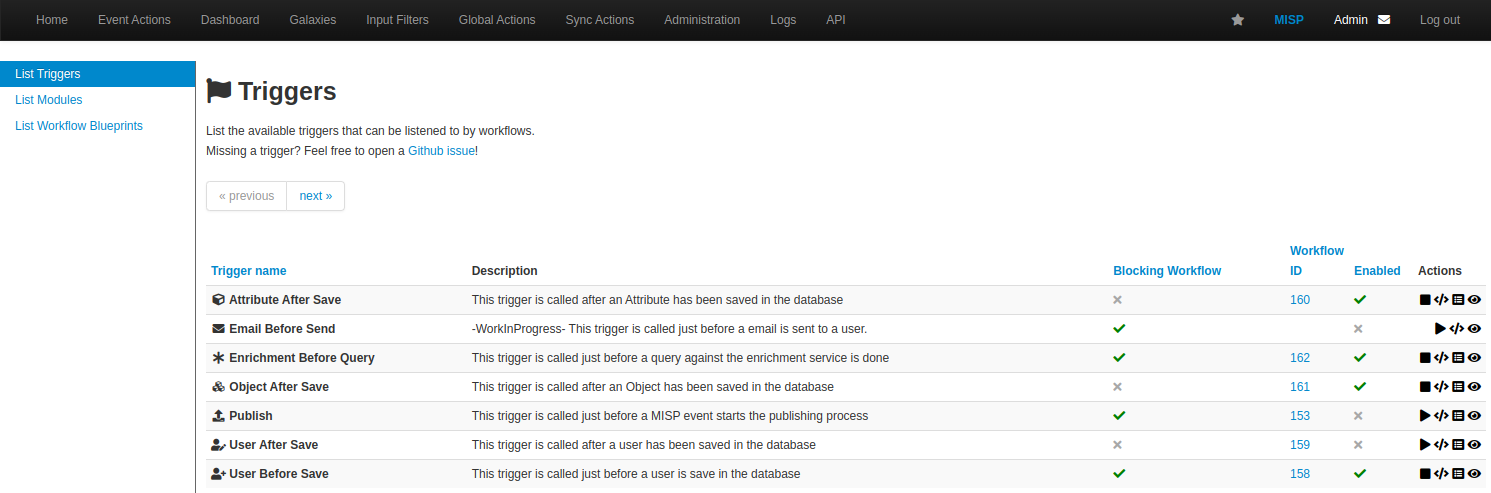
\includegraphics[width=0.8\linewidth]{pictures/usage-1.png}
    \end{center}
    \begin{center}
        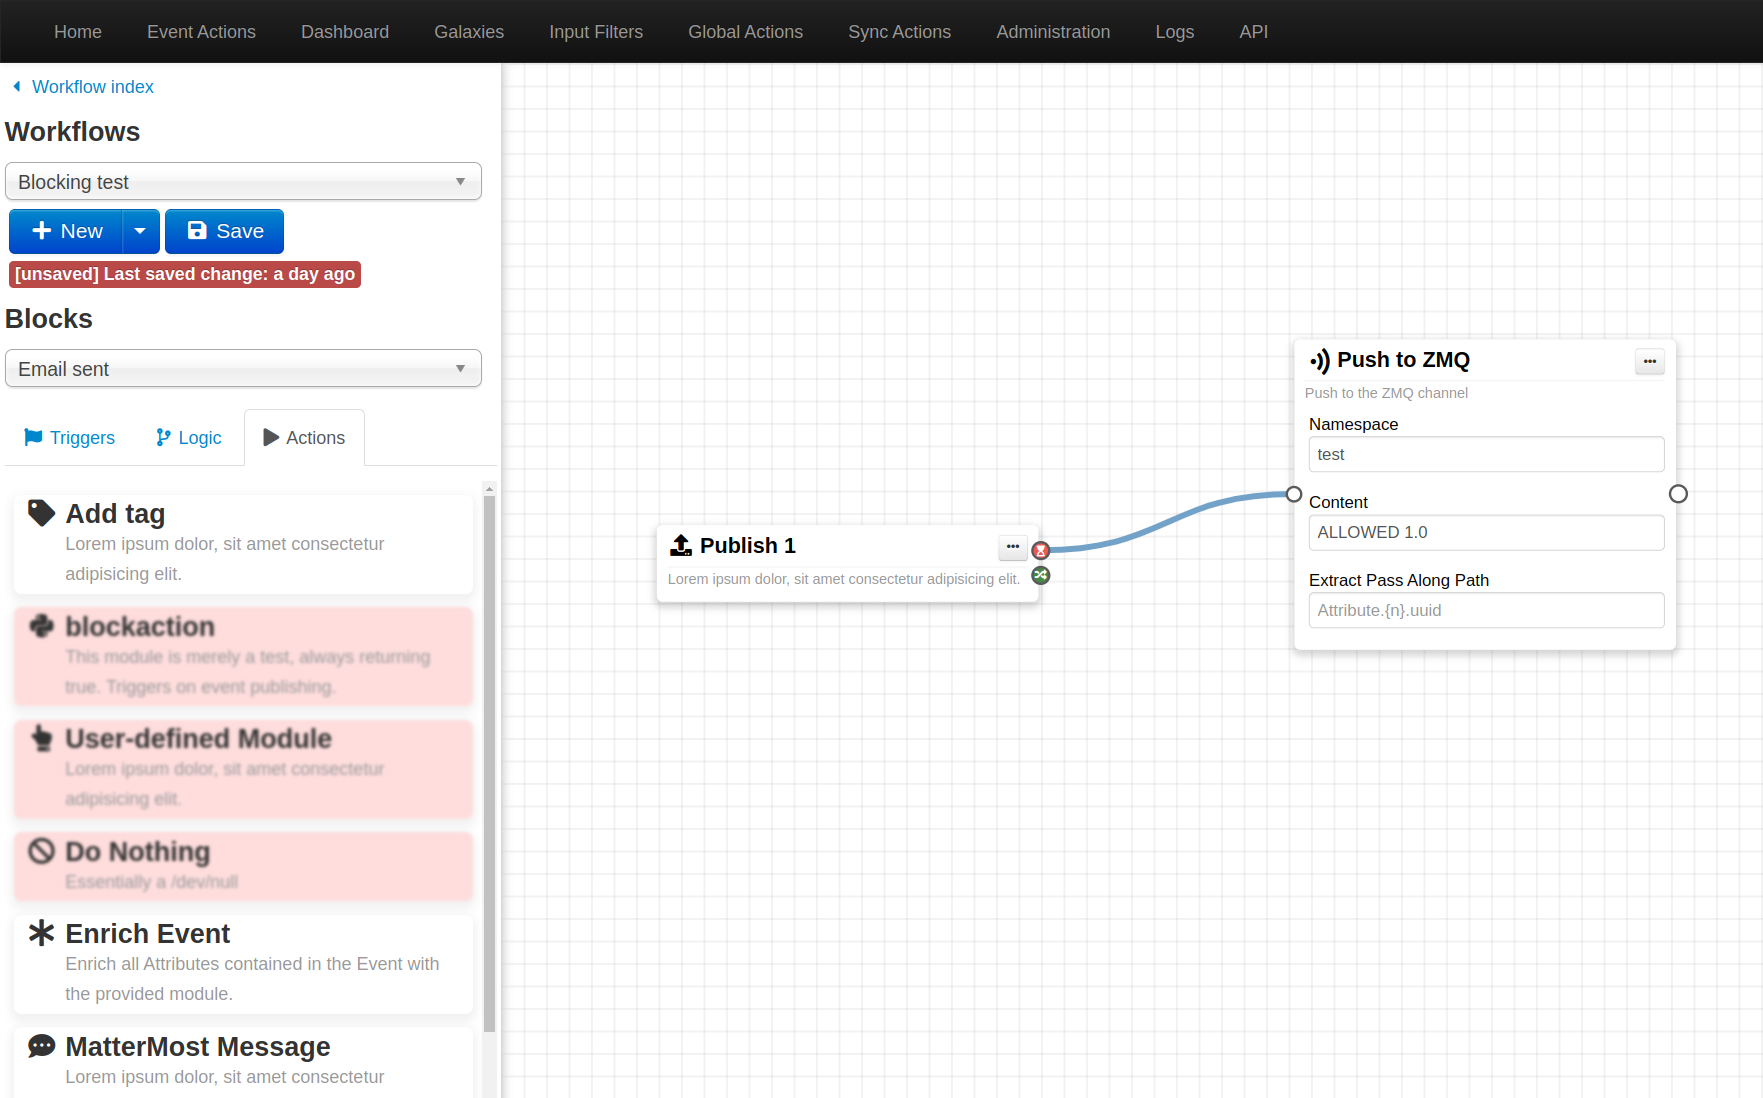
\includegraphics[width=0.50\linewidth]{pictures/editor-1.png}
    \end{center}
\end{frame}

\begin{frame}
    \frametitle{Working with the editor}
    Operations not allowed:
    \begin{itemize}
        \item Execution loop are not authorized
        \begin{itemize}
            \item Current caveat: If an action re-run the workflow in any way
        \end{itemize}
    \end{itemize}
    \begin{center}
        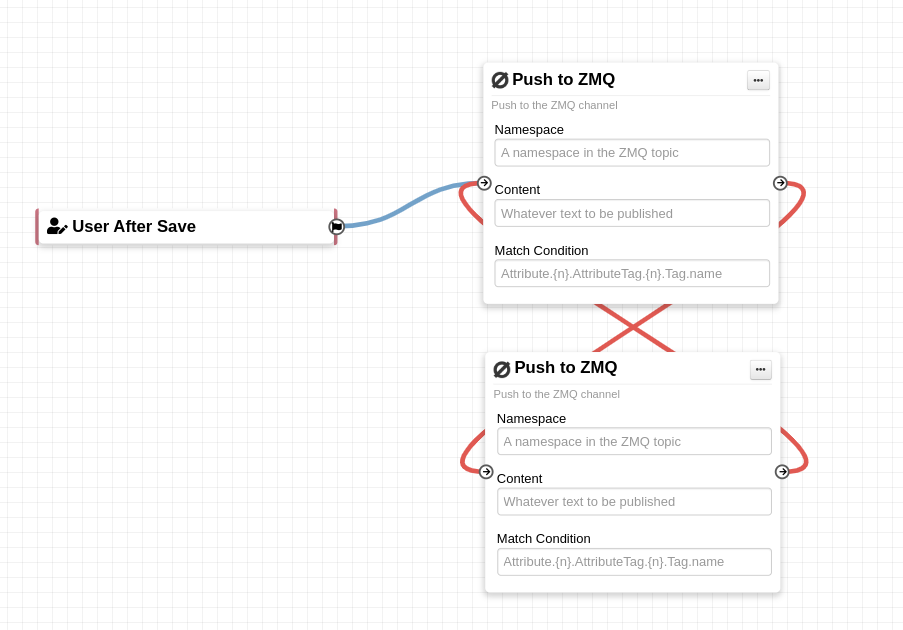
\includegraphics[width=0.7\linewidth]{pictures/editor-not-allowed-1.png}
    \end{center}
\end{frame}

\begin{frame}
    \frametitle{Workflow blueprints}
    \begin{enumerate}
        \item Blueprints allow to re-use parts of a workflow in another one
        \item Blueprints can be saved, exported and shared
    \end{enumerate}
    \begin{center}
        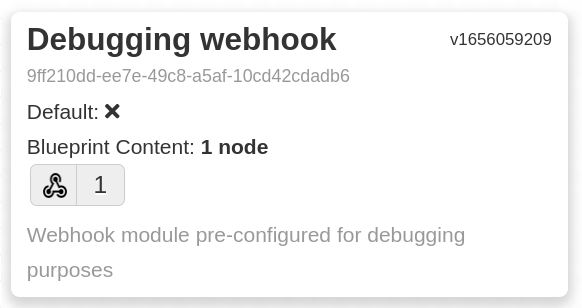
\includegraphics[width=0.5\linewidth]{pictures/blueprint-debugging.png}
    \end{center}
    Blueprints origins:
    \begin{enumerate}
        \item From the "official" \texttt{misp-workflow-blueprints} repository
        \item Created or imported by users
    \end{enumerate}
\end{frame}

\begin{frame}
    \frametitle{Workflow blueprints: Create}
    Select one or more modules to be saved as blueprint then click on the \texttt{save blueprint} button
    \begin{center}
        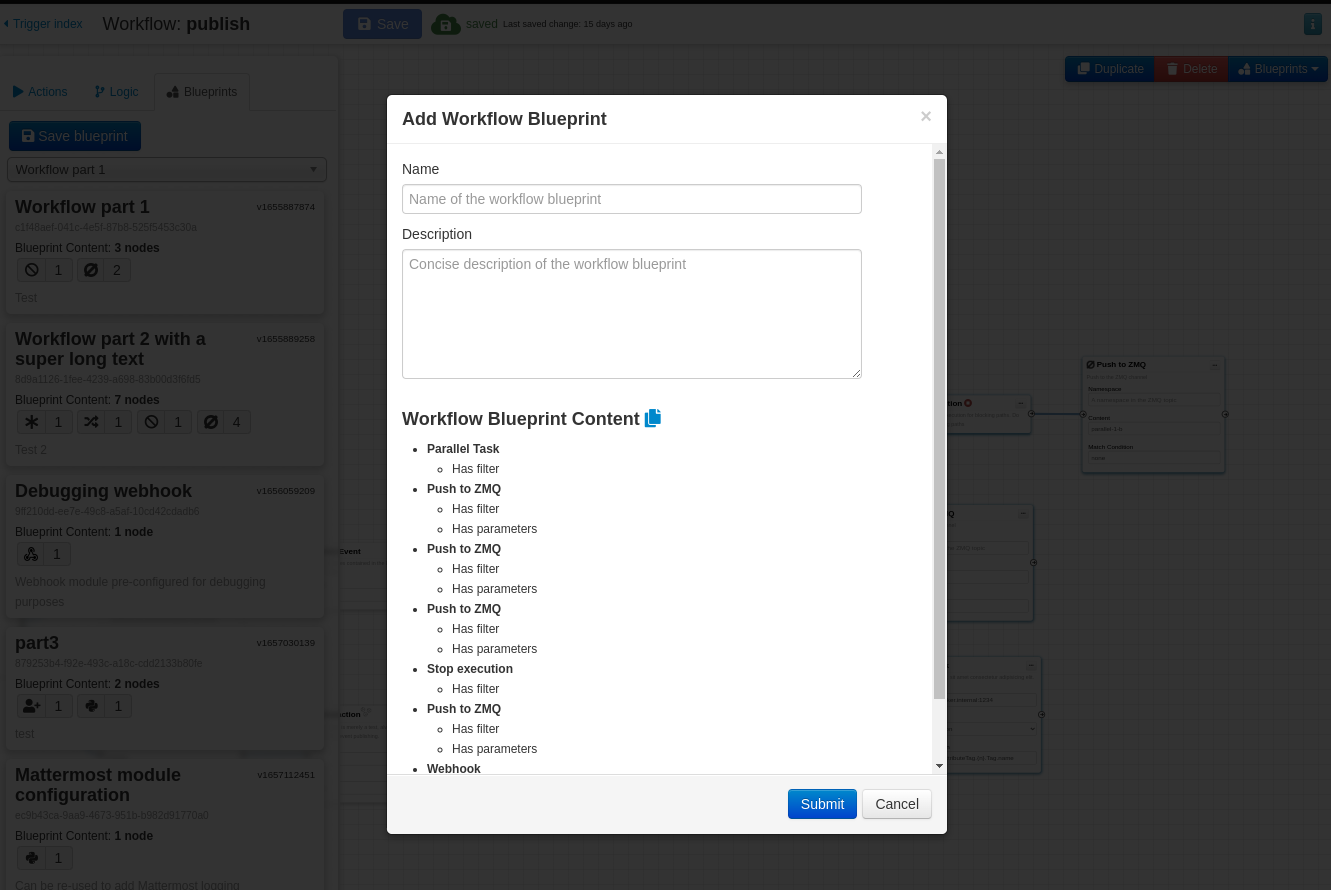
\includegraphics[width=0.85\linewidth]{pictures/blueprint-1.png}
    \end{center}
\end{frame}

\begin{frame}
    \frametitle{Module filtering}
    \begin{itemize}
        \item Some action module accept \texttt{module filtering} conditions
        \item For example, the \texttt{enrich-event} module will only perform the enrichment on Attribute having a \texttt{tlp:white} tag
    \end{itemize}
    \begin{center}
        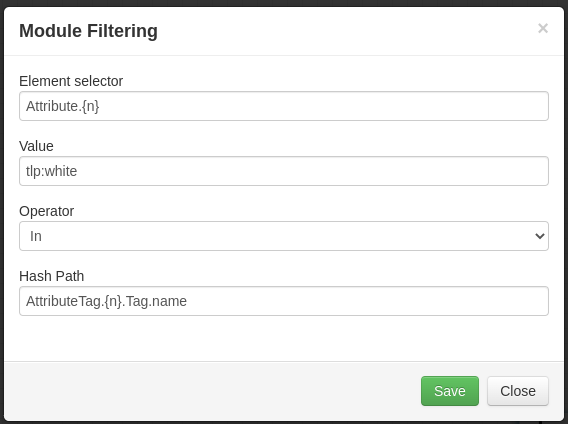
\includegraphics[width=0.7\linewidth]{pictures/module-filtering.png}
    \end{center}
\end{frame}

\begin{frame}[fragile]
    \frametitle{Hash path filtering}
    \begin{itemize}
        \item Some modules have the possibility to filter or check conditions using CakePHP's path expression.
    \end{itemize}
\begin{lstlisting}[language=javascript,firstnumber=1]
$path_expression = '{n}[name=fred].id';
$users = [
    {'id': 123, 'name': 'fred', 'surname': 'bloggs'},
    {'id': 245, 'name': 'fred', 'surname': 'smith'},
    {'id': 356, 'name': 'joe', 'surname': 'smith'},
];
$ids = Hash::extract($users, $path_expression);
// => $ids will be [123, 245]
\end{lstlisting}
\end{frame}

\begin{frame}
    \frametitle{Data format in Workflows}
    \begin{itemize}
        \item All triggers will inject data in a workflow
        \item In some cases, there is no format (e.g. User after-save)
        \item In others, the format is \textbf{compliant with the MISP Core format}
        \item In addition to the RFC, the passed data has \textbf{additional properties}
        \begin{itemize}
            \item Attributes are always encapsulated in the Event or Object
            \item Additional key \texttt{\_AttributeFlattened}
            \item Additional key \texttt{\_allTags}
            \item Additional key \texttt{inherited} for Tags
        \end{itemize}
    \end{itemize}
\end{frame}

\begin{frame}
    \frametitle{Logic module: Concurrent Task}
    \begin{itemize}
        \item Special type of \textbf{logic} module
        \item Allows breaking the execution flow into a concurrent tasks to be executed later on by a background worker
        \item As a side effect, blocking modules cannot cancel an ongoing operation anymore
    \end{itemize}
\end{frame}

\begin{frame}
    \frametitle{Debugging Workflows}
    \begin{itemize}
        \item Workflow execution is logged in the application logs: \texttt{/admin/logs/index}
        \item Or stored on disk in the following file: \texttt{/app/tmp/logs/workflow-execution.log}
    \end{itemize}
\end{frame}

\section{Learning by examples}
\begin{frame}
    \frametitle{Workflow example 1}
    \begin{center}
        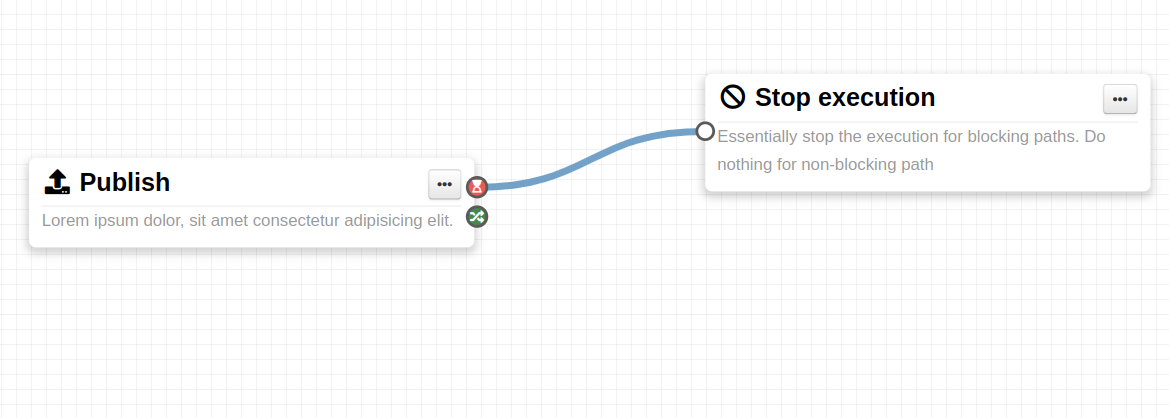
\includegraphics[width=0.95\linewidth]{pictures/example-1.png}
    \end{center}

    \begin{itemize}
        \item The \texttt{zmq} module will be run if at least one of the attribute has the \texttt{tlp:white} tag.
    \end{itemize}
\end{frame}

\begin{frame}
    \frametitle{Workflow example 2}
    \begin{center}
        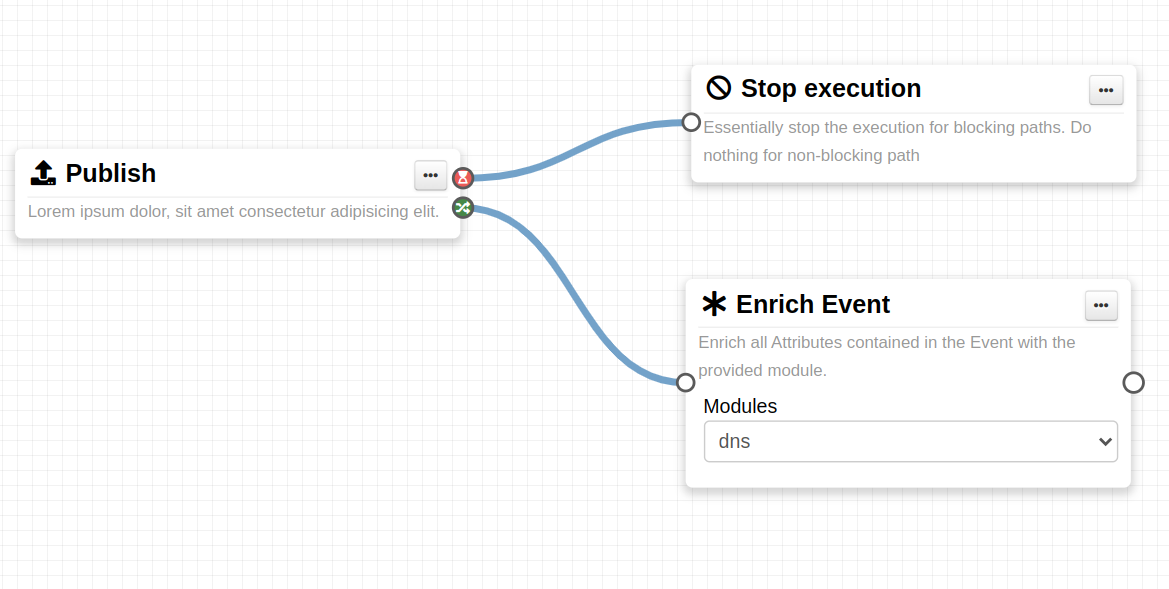
\includegraphics[width=0.95\linewidth]{pictures/example-2.png}
    \end{center}

    \begin{itemize}
        \item If an event has the \texttt{PAP:RED} tag or any of the attribute has it, the enrichment process will be cancelled
    \end{itemize}
\end{frame}

\begin{frame}
    \frametitle{Creating a new module in PHP}
    \begin{center}
        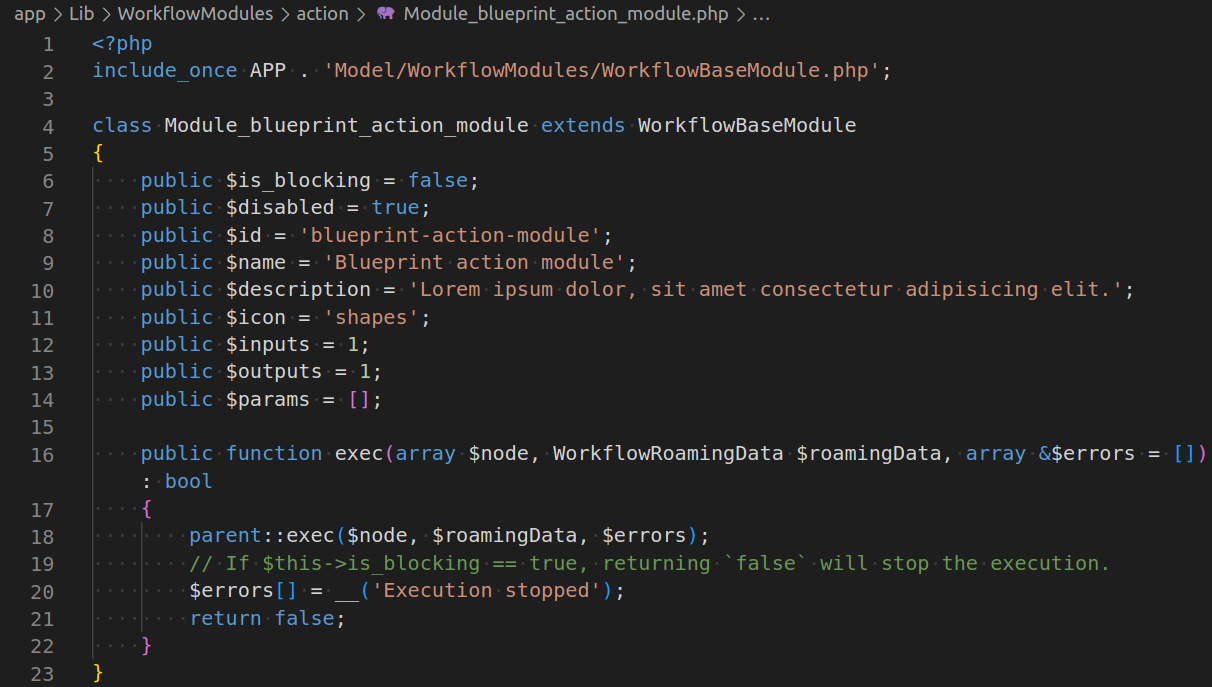
\includegraphics[width=0.65\linewidth]{pictures/custom-1.png}
    \end{center}

    \begin{itemize}
        \item Module configuration are defined as public variables
        \item The \texttt{exec} function has to be implemented.
        \begin{itemize}
            \item If it returns \texttt{true}, execution will proceed
            \item If it returns \texttt{false}
            \begin{itemize}
                \item And the module is \texttt{blocking}, the execution will stop and the operation will be blocked
                \item And the module is not \texttt{blocking}, the execution for the current path will stop
            \end{itemize}
        \end{itemize}
    \end{itemize}
\end{frame}


\begin{frame}
    \frametitle{Creating a new module in Python}
    \begin{center}
        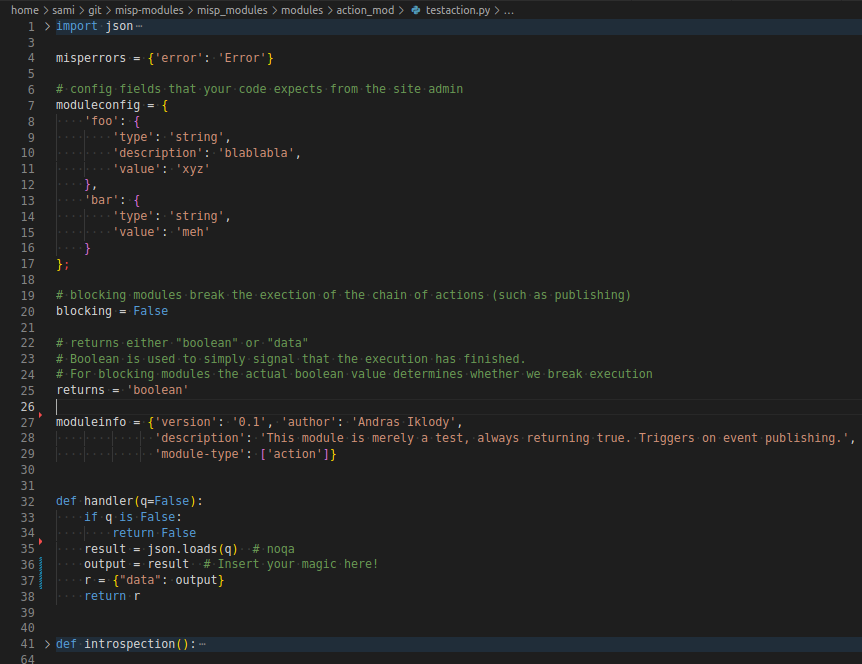
\includegraphics[width=0.6\linewidth]{pictures/custom-2.png}
    \end{center}

    \begin{itemize}
        \item Module configuration are defined in the \texttt{moduleinfo} and \texttt{moduleconfig} variables
        \item The \texttt{handler} function has to be implemented.
        \item Blocking logic is the same as other modules
    \end{itemize}
\end{frame}

